\documentclass[border=10pt]{standalone}
\usepackage{tikz}
\usetikzlibrary{arrows.meta, positioning}

\definecolor{pastelpurple}{HTML}{6E66BA}
\begin{document}
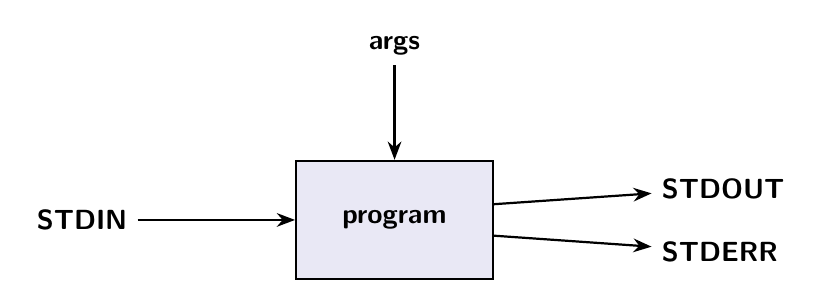
\begin{tikzpicture}[
    >=Stealth,
    thick,
    label/.style={font=\sffamily\bfseries},
    every edge/.style={draw, ->, thick}
]

% program box
\node[draw, rectangle, minimum width=2.5cm, minimum height=1.5cm, fill=pastelpurple!15, font=\sffamily\bfseries] (program) {program};

% labels
\node[label, left=2cm of program] (stdin) {STDIN};
\node[label, above=1.2cm of program] (args) {args};
\node[label, right=2cm of program, yshift=0.4cm] (stdout) {STDOUT};
\node[label, right=2cm of program, yshift=-0.4cm] (stderr) {STDERR};

% arrows
\draw[->] (stdin) -- (program);
\draw[->] (args) -- (program);
\draw[->] (program.east) ++(0,0.2) -- (stdout);
\draw[->] (program.east) ++(0,-0.2) -- (stderr);

\end{tikzpicture}
\end{document}
